\section{IP Core Growth}

	The processor's growth was analyzed in function of the parameters that it has. For this purpose, 
	processors of 8x8, 16x16 and 32x32 (places x transitions) were generated, with capacity of 7 bits 
	by place and elements of time of 48 bits. The results are plotted in Figure \ref{fig:growth}
	
	\begin{figure}[h]
			\centering
			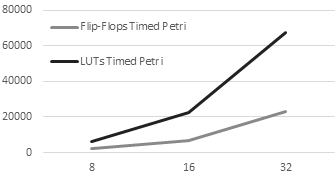
\includegraphics[width=0.95\linewidth]{./img/ipcore}
			\caption{IP Core Growth}
			\label{fig:growth}
	\end{figure}
	
	Is observed that the growth of IP Core is not something to ignore, since the number of elements 
	used grows quickly with the product of places and transitions.	 	